\chapter{Introducción}
\label{cap:introduccion}

La medición del tamaño y de la forma de los peces es una tarea habitual en la producción acuícola, porque a partir de ella se sigue el crecimiento de un lote, se estima el rendimiento y se seleccionan los ejemplares destinados a reproducción. En la práctica, estas medidas se obtienen de forma manual, lo que implica retirar al pez del agua, sujetarlo y apoyarlo sobre una regla. El procedimiento consume tiempo, requiere personal con experiencia y expone al animal a un estrés que puede provocarle lesiones \parencite{Fernandes2020,Saleh2023,Torres2018}. Por este motivo existe un interés sostenido en obtener las medidas a partir de imágenes. Sin embargo, localizar al pez dentro de la fotografía resuelve solo una parte del problema, ya que luego es necesario convertir las distancias observadas en píxeles a una longitud expresada en milímetros.

Esta conversión presenta una dificultad adicional cuando la fotografía se toma desde el exterior de un tanque. La luz que proviene del pez atraviesa el agua, la pared de vidrio y el aire antes de llegar a la cámara, y en cada cambio de medio modifica su dirección por refracción. En consecuencia, una cámara que observa a través de una interfaz aire--vidrio--agua con puerto plano no se comporta, en general, como una cámara \emph{pinhole} central, es decir, como el modelo ideal en el que todos los rayos pasan por un único punto \parencite{Agrawal2012,Treibitz2012}. El efecto práctico es que el tamaño aparente del pez depende de la distancia que lo separa del vidrio, y esa distancia no puede determinarse a partir de una sola imagen. La calibración de la cámara realizada directamente bajo el agua compensa parte de este efecto en la zona donde se efectuó la calibración, pero el error varía a medida que el objeto se aleja de ella \parencite{Rofallski2022}. La Figura~\ref{fig:1-1} muestra la geometría del problema: el rayo que llega al sensor se desvía en las dos caras del vidrio, de modo que la posición aparente del punto depende de la distancia cámara--vidrio, del espesor del vidrio y de la profundidad del punto.

\begin{figure}[H]
\centering
\caption[Configuración conceptual de cámara, vidrio, agua y rayos refractados]{Configuración conceptual de cámara, vidrio, agua y rayos refractados. El rayo que llega al sensor desde el punto $P$ se quiebra en las interfaces $\pi_1$ y $\pi_2$, de modo que el píxel «ve» el punto en un lugar distinto del que ocupa; el desplazamiento depende de la distancia $d$, del espesor $t_g$ y de la profundidad $z$ del punto detrás del vidrio.}
\label{fig:1-1}
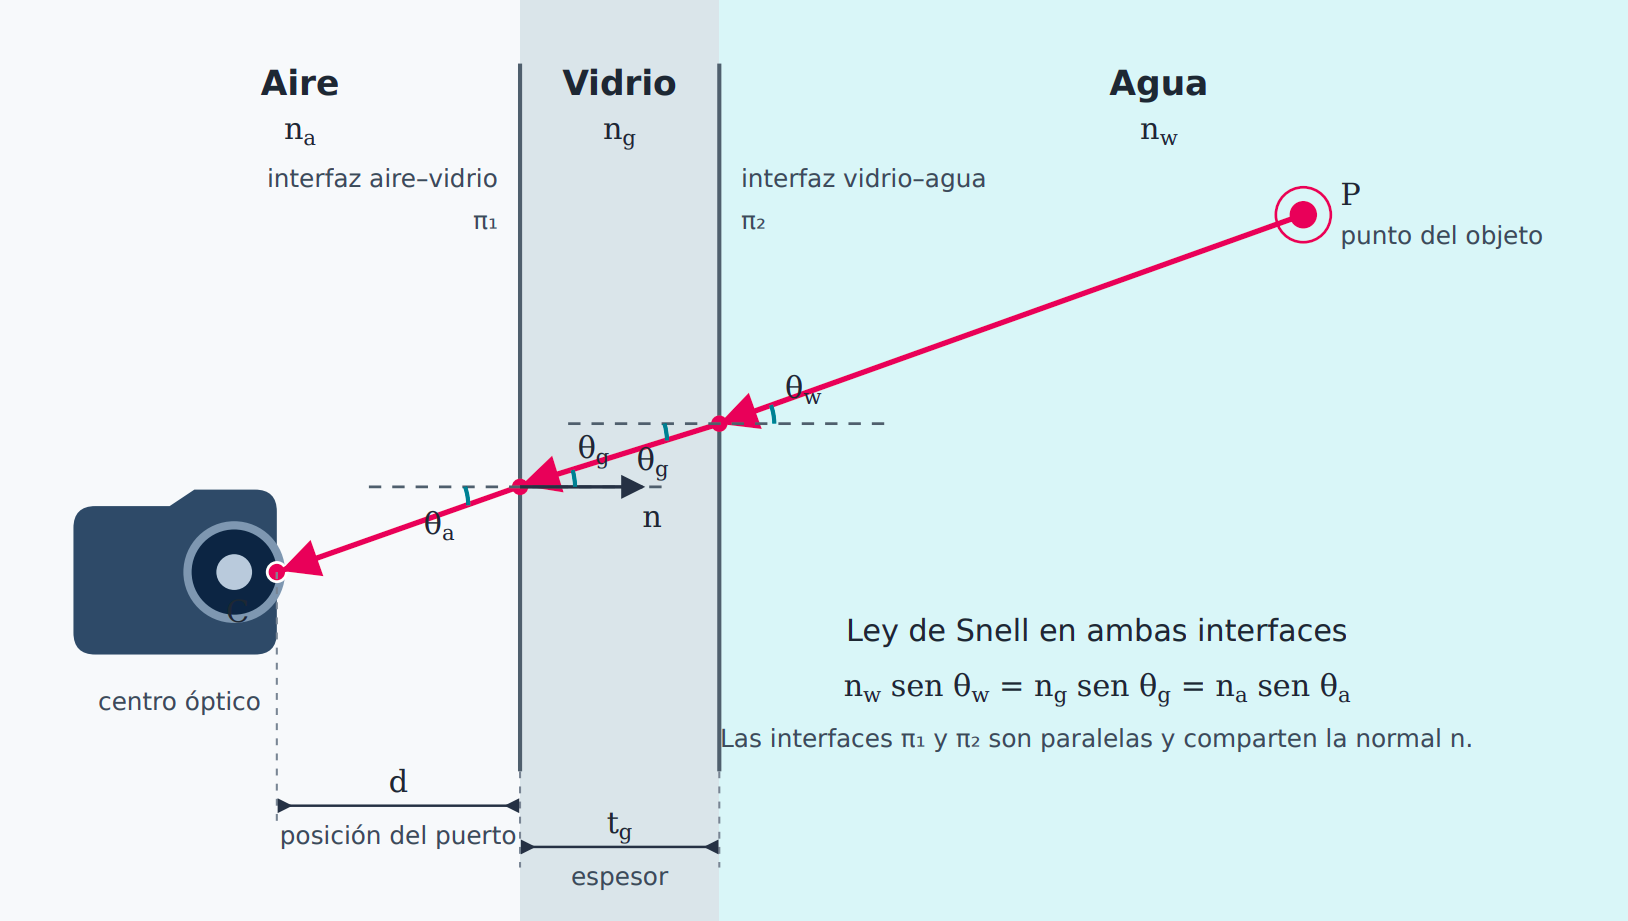
\includegraphics[width=0.9\textwidth]{fig1_1_configuracion.png}
\fignota{Elaboración propia.}
\end{figure}

En este trabajo se evaluaron cuatro procedimientos para convertir píxeles en milímetros, aplicados a los mismos puntos anatómicos de la misma imagen. El primero (A) utiliza la escala de un marcador ArUco adherido al vidrio. El segundo (\Aprime) emplea una homografía calculada con un marcador ubicado en el mismo plano que la réplica. El tercero (B) corresponde a una calibración \emph{pinhole} efectiva realizada bajo el agua. El cuarto (C) modela de forma explícita la desviación de los rayos en el puerto plano. En lugar de peces vivos se utilizaron réplicas rígidas medidas con calibre, de manera que cada estimación pudiera compararse con una longitud conocida. Cuando la profundidad era conocida, se comparó el error de las cuatro rutas; cuando se la consideró desconocida, se empleó C para calcular el intervalo de longitudes compatible con cualquier posición dentro de la pecera y determinar cuánto debe acotarse la profundidad para que ese intervalo resulte útil.



El tema surgió de una pregunta práctica: de qué manera pasar de píxeles a milímetros cuando se quiere medir un pez en una pecera con una cámara convencional. Las respuestas disponibles en la bibliografía son un marcador de escala, una calibración realizada bajo el agua o un modelo óptico explícito, y cada una produce un valor distinto para la misma fotografía. Los trabajos revisados muestran que la refracción afecta la medición \parencite{Agrawal2012,Rofallski2022,Treibitz2012}, pero no comparan el error de estas alternativas sobre los mismos puntos y contra una referencia física cuando la cámara se ubica del lado exterior de un vidrio plano (Sección~\ref{sec:antecedentes}).

Se estudió, por lo tanto, un flujo de medición con una sola cámara y puntos anatómicos marcados a mano sobre fotografías de réplicas rígidas tomadas a través de una pecera de vidrio. Se compararon las cuatro rutas de conversión, A, \Aprime, B y C, sobre los mismos puntos de cada imagen y se evaluó cada una contra la medida física de la réplica. El tema reúne conocimientos de visión por computadora, geometría proyectiva y metrología. Desde la perspectiva de la Ingeniería Informática, el aporte consiste en un procedimiento de medición monocular que declara de forma explícita la incertidumbre que introduce el desconocimiento de la profundidad, y en un módulo de trazado refractivo implementado y verificado experimentalmente.

\section{Enunciado del problema}
\label{sec:enunciado}

\subsection{Planteamiento del problema}

Diversos trabajos han demostrado que de una imagen pueden extraerse tanto los puntos anatómicos de un pez como una referencia de escala, ya sea mediante algoritmos o de forma manual \parencite{Correia2025,Saleh2023,Tseng2020}. Los primeros enfoques se desarrollaron fuera del agua o en montajes controlados. \textcite{Monkman2019} detectaron el pez junto con un marcador ArUco colocado a su lado, aproximadamente en el mismo plano; \textcite{Fernandes2020} segmentaron imágenes de tilapia para extraer medidas corporales; y \textcite{Saleh2023} localizaron puntos anatómicos con fines morfométricos. Estos estudios confirman que las imágenes contienen información morfométrica aprovechable. Muestran también que la correcta ubicación de los puntos no es suficiente para obtener una medida física exacta, y ninguno de ellos considera lo que ocurre cuando la imagen se forma a través de una pared de vidrio y la escala varía con la profundidad.

En condiciones subacuáticas se agrega una dificultad, dado que además de localizar al pez es necesario recuperar su escala o su profundidad. \textcite{AlJubouri2017} resolvieron este problema con dos cámaras ortogonales, y \textcite{Zhou2023} y \textcite{Seibold2026}, mediante visión estéreo y triangulación. MorphoCal emplea una sola cámara, aunque sumergida, y proyecta los puntos sobre un plano de referencia definido mediante una calibración \emph{pinhole} realizada bajo el agua \parencite{Vijayalakshmi2026}. \textcite{Yin2026} corrigieron la refracción en una interfaz aire--agua y analizaron el efecto de suponer distintas profundidades, pero trabajaron con una profundidad nominal y no informaron un intervalo de longitud. Pinax y CalibMar modelan puertos planos, aunque no fueron concebidos para medir peces \parencite{Luczynski2017,Seegraber2025}. En la bibliografía revisada no se encontró una evaluación monocular que compare A, \Aprime, B y C sobre los mismos puntos y que, además, cuantifique el intervalo de longitud cuando la profundidad es desconocida. La Sección~\ref{sec:antecedentes} desarrolla estos antecedentes y los compara en detalle.


La medición a partir de imágenes permitiría reducir la manipulación de los animales y observarlos con mayor frecuencia. El obstáculo es de naturaleza física: cuando la escena atraviesa la interfaz aire--vidrio--agua, la cámara deja de comportarse como una cámara perspectiva simple, y la refracción, sumada a la diferencia de profundidad entre el pez y el marcador de escala, puede producir una longitud aparente distinta de la real aunque los cuatro puntos anatómicos estén correctamente marcados.

La dificultad metodológica consiste en separar tres efectos que suelen presentarse combinados: la escala directa de un marcador adherido al vidrio, la calibración aproximada de una cámara bajo el agua y el modelado explícito de los rayos a través del puerto plano. Para aislarlos, se compararon las rutas A, \Aprime, B y C en la misma imagen y sobre los mismos puntos anatómicos, y se evaluó además la ruta C sobre todo el rango de profundidades físicamente posibles. El resultado de esta última evaluación es un rango geométrico y no un intervalo de confianza estadístico: $[\min_{z} L(z), \max_{z} L(z)]$, es decir, el conjunto de longitudes compatibles con desconocer la posición de $z$ dentro de $[z_{\min}, z_{\max}]$. La notación abreviada $[L(z_{\min}), L(z_{\max})]$ solo es válida cuando $L(z)$ es monótona en ese intervalo.

El estudio se limita a réplicas rígidas vistas de perfil y a dos medidas, la longitud total y la profundidad corporal, esta última tomada sobre el cuerpo y sin incluir las aletas. Los cuatro puntos anatómicos se marcaron a mano una sola vez sobre cada imagen original y se reutilizaron en las cuatro rutas. Las capturas repetidas de una misma réplica se consideran repeticiones técnicas y no unidades experimentales independientes. Esta delimitación permitió aislar el efecto geométrico, a costa de no poder extender las conclusiones de manera directa a peces vivos, en movimiento, en agua turbia, parcialmente ocultos o en posturas distintas de la de perfil.

De esta brecha y de esta delimitación surgen las preguntas que orientaron la investigación.

\subsection{Formulación del problema}

El problema se formula mediante una pregunta principal y dos preguntas secundarias.

\subsubsection*{Pregunta principal}

¿Qué rango de longitudes produce la ruta C al variar la profundidad $z$ dentro del rango físicamente admisible de la pecera y de ventanas acotadas de $\pm 3$ y $\pm 1$~cm, y qué ancho relativo y qué cobertura de la referencia se observan en el montaje experimental?

\subsubsection*{Preguntas secundarias}

\begin{enumerate}
  \item Con $z$ conocida, ¿cómo se comportan A, \Aprime, B y C en longitud total y en profundidad corporal, y cómo cambia el error de A y de B al alejarse de la zona de calibración de B?
  \item ¿Qué sensibilidad tiene la estimación de C a los parámetros geométricos del montaje medidos a mano (distancia cámara--vidrio e índice de refracción del agua)?
\end{enumerate}

\section{Objetivos de la investigación}

\subsection{Objetivo general}

Evaluar, en un montaje controlado con una interfaz aire--vidrio--agua, cuatro estrategias de conversión métrica para estimar con una sola cámara la longitud total y la profundidad corporal de peces, comparándolas sobre los mismos puntos anatómicos contra referencias físicas de réplicas rígidas, y cuantificar con un modelo refractivo de puerto plano el intervalo de longitud que introduce una profundidad desconocida.

\subsection{Objetivos específicos}

\begin{enumerate}
  \item Construir y documentar el conjunto de datos de réplicas, referencias físicas, posiciones, repeticiones y exclusiones.
  \item Establecer un protocolo reproducible de marcado manual de los cuatro puntos anatómicos, único por imagen y compartido por las cuatro rutas.
  \item Implementar y validar las rutas A, \Aprime, B y C, incluido el módulo C de puerto plano, frente a las referencias físicas de las réplicas.
  \item Comparar el error de longitud total y de profundidad corporal de A, \Aprime, B y C sobre las mismas imágenes, y analizar cómo varía ese error con la distancia de la réplica al vidrio.
  \item Calcular el intervalo $[\min_z L(z), \max_z L(z)]$ sobre el rango físicamente admisible de profundidad y sobre ventanas acotadas de $\pm 3$ y $\pm 1$~cm, junto con su ancho relativo y su cobertura.
  \item Evaluar la sensibilidad de las estimaciones de C a las condiciones geométricas del montaje medidas a mano (distancia cámara--vidrio e índice de refracción del agua).
\end{enumerate}

Los objetivos 1, 2 y 3 construyen el conjunto de datos, el protocolo de marcado y las rutas sobre las que se trabaja; el objetivo 4 responde a la pregunta secundaria 1 y se contrasta con las hipótesis H1 y H2; el objetivo 5 responde a la pregunta principal y se contrasta con la hipótesis H3; y el objetivo 6 responde a la pregunta secundaria 2 (Sección~\ref{sec:hipotesis}). Las conclusiones del Capítulo~5 se presentan en ese mismo orden.

\section{Hipótesis}
\label{sec:hipotesis}

Se plantean tres hipótesis de investigación. Los criterios con que se decide cada una se definen en la Sección~\ref{sec:criterios-hipotesis}.

\begin{description}
  \item[H1: comparación geométrica con profundidad conocida.] Con la profundidad conocida, el error absoluto de longitud total de C es menor que el de A, \Aprime{} y B. Responde a la pregunta secundaria 1 y a los objetivos 3 y 4.
  \item[H2: dependencia con la distancia.] La diferencia $\mathrm{error}(B) - \mathrm{error}(C)$ aumenta con la separación respecto de la zona de calibración de B. Responde a la pregunta secundaria 1 y al objetivo 4.
  \item[H3: intervalo por profundidad desconocida.] El intervalo calculado con C, $\IL = [\min_z L(z), \max_z L(z)]$, contiene la longitud física de la réplica cuando $z$ recorre el rango físicamente admisible, y su ancho relativo puede predecirse a partir de la geometría del montaje ($d$, $t_g$, índices y rango de $z$). Responde a la pregunta principal y al objetivo 5.
\end{description}

\section{Justificación}

La medición repetible de los peces permite seguir su crecimiento, estimar el rendimiento y seleccionar ejemplares. En Paraguay la actividad tiene una escala que justifica el interés en el tema, dado que la acuicultura produjo alrededor de 14\,000 toneladas en 2021 \parencite{FAO2025Paraguay}. Un sistema basado en imágenes podría reducir la manipulación directa de los animales y permitir observaciones más frecuentes.

Para la Ingeniería Informática, el interés radica en determinar el límite métrico de un procedimiento con una sola cámara cuando la escena atraviesa un puerto plano. Se mantuvieron fijos la imagen y los cuatro puntos marcados a mano, se compararon A, \Aprime, B y C sobre las mismas observaciones y se hizo explícita la incertidumbre geométrica que agrega la profundidad. El resultado es evidencia experimental que permite decidir en qué condiciones es suficiente una escala directa, cuándo conviene una calibración \emph{pinhole} y cuándo se requiere un modelo refractivo.

La contribución puede verificarse en cinco aspectos: una salida monocular que declara la incertidumbre atribuible a la profundidad; evidencia comparativa de A, \Aprime, B y C en un montaje controlado; una implementación propia del modelo de puerto plano, basada en formulaciones publicadas y evaluada contra referencias físicas; un protocolo reproducible de marcado manual con réplicas rígidas; y un análisis de la sensibilidad de C a los parámetros del montaje medidos a mano.

\section{Delimitación espacial y temporal}
\label{sec:delimitacion}

El trabajo se desarrolló en \Ciudad, Paraguay, sobre un montaje experimental propio: una pecera de vidrio de $30 \times 30 \times 30$~cm, una cámara de teléfono fija y seis réplicas rígidas de peces, descritos en el Capítulo~\ref{cap:metodologia}. Los resultados se refieren a ese montaje. En lo temporal, el trabajo abarcó de agosto a octubre de 2026: armado del montaje y pruebas preliminares en agosto y septiembre, capturas definitivas y calibraciones de cámara en octubre de 2026, y búsqueda de antecedentes cerrada en septiembre de 2026.

\section{Alcance y limitaciones}
\label{sec:alcance}

El trabajo evalúa de forma comparativa cuatro rutas de conversión métrica con una sola cámara y cuantifica la incertidumbre geométrica que introduce una profundidad desconocida. Los resultados corresponden a réplicas rígidas fotografiadas de perfil, en un montaje controlado y con los índices de refracción adoptados en el Capítulo~\ref{cap:metodologia}.

Quedan fuera del alcance los peces vivos, el agua turbia, el movimiento, las oclusiones y las instalaciones productivas. El marcado de los puntos anatómicos es manual, y la repetibilidad del operador no se cuantificó; su posible efecto sobre las medidas se discute en la Sección~\ref{sec:limitaciones}.

\section{Estructura del documento}

El documento consta de cinco capítulos, ordenados según la estructura que establece el reglamento de Proyecto Final de Carrera para una investigación.

\begin{description}
  \item[Capítulo 1. Introducción.] Presenta la motivación, el enunciado del problema con su planteamiento y sus preguntas, los objetivos, las hipótesis, la justificación, la delimitación espacial y temporal, el alcance y las limitaciones, y la estructura del documento.
  \item[Capítulo 2. Marco teórico.] Reúne los antecedentes y la brecha de investigación; el marco referencial, que explica la morfometría, la formación de imágenes a través de una interfaz plana, las rutas A, \Aprime, B y C, el marcado manual, los marcadores ArUco y la evaluación de mediciones; y el marco conceptual, con las definiciones de los términos principales.
  \item[Capítulo 3. Marco metodológico.] Describe el tipo y el enfoque de la investigación, la población y la muestra, las variables con su definición conceptual y operacional, los criterios de decisión de las hipótesis, los instrumentos y técnicas de recolección de datos, los métodos de conversión, el procedimiento, el análisis y la trazabilidad del experimento.
  \item[Capítulo 4. Presentación, análisis e interpretación de resultados.] Presenta los datos y las exclusiones, las calibraciones, la comparación entre A, \Aprime, B y C, el comportamiento según la profundidad, el intervalo por profundidad desconocida, el contraste de hipótesis y la discusión.
  \item[Capítulo 5. Conclusiones y recomendaciones.] Ofrece la regla de decisión que resume el aporte, una conclusión por objetivo, el impacto potencial, las limitaciones, las recomendaciones y el trabajo futuro.
\end{description}

Los anexos reúnen el registro visual de las capturas, los parámetros del puerto plano, los perfiles de calibración, la referencia geométrica del riel, el índice de los repositorios de código y datos, la tabla maestra de resultados, las fichas de las réplicas y las fotografías del montaje y de los instrumentos.
